In signal processing, we follow the Nyquist rate $f_{Nyq}=\frac{1}{2\Delta t}$ in sampling signals in order to avoid aliasing. However, sampling at least twice the maximum signal frequency could lead to high surveying and time costs. There are two approaches to address this challenge: compressive sampling and data interpolation. Compressive sampling (CS) leverages the principles of sparsity, which relates to the signals of interest, and incoherence, which relates to the sensing modality \cite{candes2008introduction}. CS theory allows accurate recovery of signals from a significantly reduced set of samples, compared to the traditional Nyquist rate, by sampling only $O(S\log{(n/S)})$ projections. \cite{candes2008introduction} In this study, our focus is on interpolation methods. These methods spatially transform irregularly sampled traces to any desired grid \cite{kaur2021seismic}. There are two major categories of seismic interpolation methods: wave equation methods and signal processing methods \cite{naghizadeh2011seismic,kaur2019seismic,kaur2021seismic}.
\\\\
Wave equation methods are based on seismic wave propagation, which requires prior knowledge of the direction of lateral coherence of the event. A velocity model is a prerequisite for interpreting traces \cite{ronen1987wave}. Given an accurate velocity model, wave-equation-based approaches can interpolate waves passing through complex geological structures and subsurface heterogeneities. Parabolic and hyperbolic events can be recovered. However, subsurface velocity models might not be present for the surveying area. These methods also employ a straight-raypath approximation, which might collapse for low-frequency waves \cite{stolt2002seismic}.
\\\\
Signal processing methods include domain transform methods or prediction filter methods. No subsurface information is required to perform traces interpolation. Multiple studies have outlined other benefits of using signal processing methods: F-X domain interpolation is insensitive to random noises \cite{spitz1991seismic}, F-K domain interpolation can preserve amplitude and perform artifact-free denoise \cite{naghizadeh2011seismic}, fast generalized Fourier transform (FTFG) can handle non-stationary seismic data \cite{naghizadeh2012seismic}, and 3D sparse time-domain Radon interpolator (TDRI) can reconstruct events with high continuity \cite{schonewille2014comparison}. The major drawback is the sparsity and linearity assumptions in the t-x domain, making these methods intolerant to highly curved or dispersed events \cite{spitz1991seismic, naghizadeh2011seismic, naghizadeh2012seismic}.
\\\\
Deep learning methods come without the aforementioned assumptions, and they do not require any velocity model. Convolutional neural networks (CNNs) combine domain transforms and prediction filter methods but without the linearity assumptions or time/frequency transforms \cite{oliveira2018interpolating}. Transforms and filters are learned and applied to the neural networks through an iterative training process. Figure \ref{fig:methods} shows different algorithms that have been exploited for seismic traces interpolation, such as CNNs, generative adversarial networks (GANs), and auto-encoders \cite{khosro2023machine}. These deep learning methods yield high reconstruction accuracy even on steep events and can be easily applied to 3D data, but they require a large amount of training data \cite{kaur2019seismic, kaur2021seismic, khosro2023machine}.
\\\\
In this study, our primary focus is on GANs. The upcoming chapters will delve into the theory behind GANs and explore neural network architectures. Due to the complexity and computational demands of seismic datasets, we decided to simulate the nature of seismic problem using more manageable 28x28 pixel MNIST and Fashion-MNIST datasets. These datasets were augmented by introducing masked columns, mimicking the missing trace scenario encountered in seismic datasets. We employ three GANs, namely Linear model, LeNeT-5, and U-NET, to reconstruct MNIST and Fashion-MNIST images. Our evaluation involves qualitative assessments and examination of validation losses.

\begin{figure}[H]
    \centering
    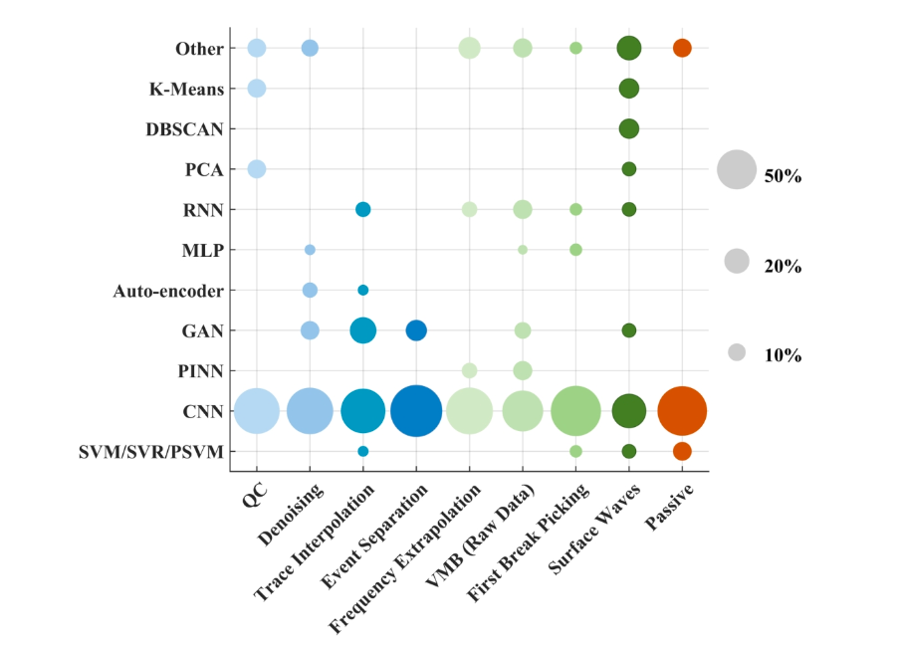
\includegraphics[width=0.8\textwidth]{Figure/Front_page/methods.png}
    \caption{\textit{Machine learning algorithms used for most prominent seismic processing applications \cite{khosro2023machine}}}
    \label{fig:methods}
\end{figure}

